\documentclass{beamer}
%
% Choose how your presentation looks.
%
% For more themes, color themes and font themes, see:
% http://deic.uab.es/~iblanes/beamer_gallery/index_by_theme.html
%
\mode<presentation>
{
  \usetheme{Boadilla}      % or try Darmstadt, Madrid, Warsaw, ...
  \usecolortheme{beaver} % or try albatross, beaver, crane, ...
  \usefonttheme{default}  % or try serif, structurebold, ...
  \setbeamertemplate{navigation symbols}{}
  \setbeamertemplate{caption}[numbered]
  
} 

\usepackage{xcolor,colortbl}
\usepackage[english]{babel}
\usepackage[utf8x]{inputenc}
\usepackage{courier}
\usepackage{dsfont}
\usepackage{verbatim} 
\usepackage{enumerate}
\usepackage{tikz}
\usetikzlibrary{shapes.geometric, arrows}
\usepackage{multirow}
\usepackage{venndiagram}
\usepackage{epigraph} 
%\usepackage{xcolor}
\usepackage{makecell}

%\usepackage{enumitem}

\usepackage{hyperref}
\hypersetup{
    colorlinks=true,
    linkcolor=blue,
    filecolor=magenta,      
    urlcolor=cyan,
}

% R stuff!
\usepackage{listings}
\definecolor{codegreen}{rgb}{0,0.6,0}
\definecolor{codegray}{rgb}{0.5,0.5,0.5}
\definecolor{codepurple}{rgb}{0.58,0,0.82}
\definecolor{backcolour}{rgb}{0.95,0.95,0.92}

\lstdefinestyle{mystyle}{
    backgroundcolor=\color{backcolour},    
    commentstyle=\color{codegreen},
    keywordstyle=\color{black},
    numberstyle=\tiny\color{codegray},
    stringstyle=\color{codepurple},
    basicstyle=\ttfamily\footnotesize,
    breakatwhitespace=false,         
    breaklines=true,                 
    captionpos=b,                    
    keepspaces=true,                 
    numbers=left,                    
    numbersep=5pt,                  
    showspaces=false,                
    showstringspaces=false,
    showtabs=false,                  
    tabsize=2
}

\lstset{style=mystyle}


\setbeamertemplate{enumerate items}[default]
\setbeamertemplate{itemize item}[triangle]

%\setitemize{label=\usebeamerfont*{itemize item}%
%  \usebeamercolor[fg]{itemize item}
%  \usebeamertemplate{itemize item}}
\tikzstyle{startstop} = [rectangle, rounded corners, 
minimum width=3cm, 
minimum height=1cm,
text centered, 
draw=black, 
fill=red!30]

\tikzstyle{io} = [trapezium, 
trapezium stretches=true, % A later addition
trapezium left angle=70, 
trapezium right angle=110, 
minimum width=3cm, 
minimum height=1cm, text centered, 
draw=black, fill=blue!30]

\tikzstyle{process} = [rectangle, 
minimum width=3cm, 
minimum height=1cm, 
text centered, 
text width=3cm, 
draw=black, 
fill=orange!30]

\tikzstyle{decision} = [diamond, 
minimum width=3cm, 
minimum height=1cm, 
text centered, 
draw=black, 
fill=green!30]
\tikzstyle{arrow} = [thick,->,>=stealth]


\title[Introduction to Statistics]{Hypothesis Testing}
\subtitle{More on Null Distributions and P-values}
\author{Grinnell College}
\date{}

\graphicspath{{img/}}

\begin{document}

\begin{frame}
  \titlepage
\end{frame}

%%%%%%%%%%%%%%%%%%%%%%%%%%%%%%%%%%%%%%%%%%%%%%%%%%%%%%%%%%%%%%%%%
\begin{frame}{Review}
\textbf{Hypothesis Testing:} formal technique for answering a question with two competing possibilities \vspace{6mm}

\textbf{Null Hypothesis:} represents a skeptical view or a perspective of no difference
\begin{itemize}
    \item H$_0$: 'parameter' = (some value)
\end{itemize}\vspace{6mm}

\textbf{Alternate Hypothesis:} what the researchers actually want to show with the study
\begin{itemize}
    \item H$_A$: 'parameter'  [$</>/\neq$]  (some value)
    \item choose the sign to match the research question
    \item both hypotheses use the same value
\end{itemize}
\end{frame}

%%%%%%%%%%%%%%%%%%%%%%%%%%%%%%%%%%%%%%%%%%%%%%%%%%%%%%%%%%%%%%%%%
\begin{frame}{Review}
This is the general outline we will follow for Hypothesis Testing \vspace{1mm}
\begin{enumerate}
    \item Define hypotheses
    \item Simulate what the parameter looks like under H$_0$
    \item See how our statistic compares to this
    \item Compute a p-value
    \begin{itemize}
        \item do the results look unlikely if H$_0$ is true?
    \end{itemize}
    \item Interpretations / Conclusions
\end{enumerate} \vspace{12mm}

\textbf{Note:} Points 2 and 3 can be combined with the creation of a something called a 'test-statistic'
\end{frame}

%%%%%%%%%%%%%%%%%%%%%%%%%%%%%%%%%%%%%%%%%%%%%%%%%%%%%%%%%%%%%%%%%
\begin{frame}{Null Distribution}
\textbf{Null Distribution} 

The distribution of the statistics if the null hypothesis is true
\begin{itemize}
    \item simulates what the null hypothesis looks like
    \item use this to compute p-values
\end{itemize} \vspace{2mm}

We looked at the coin-flip scenario. Null distribution of fair coin, 10 flips

\begin{center}
    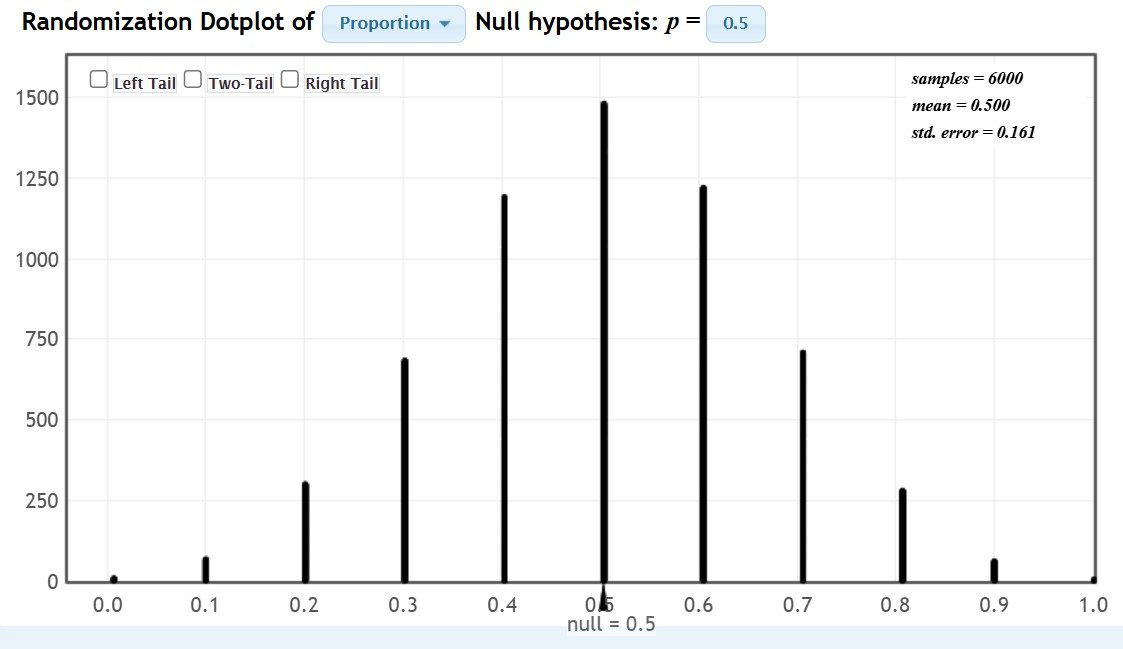
\includegraphics[scale=.42]{img/coin_null_distr.jpg}
\end{center}

\end{frame}

%%%%%%%%%%%%%%%%%%%%%%%%%%%%%%%%%%%%%%%%%%%%%%%%%%%%%%%%%%%%%%%%%
\begin{frame}{Null Distribution}
What if we flipped 100 coins instead of 10
\begin{itemize}
    \item Would getting $\hat{p} = .8$ be more common or less common?
\end{itemize}
\end{frame}

%%%%%%%%%%%%%%%%%%%%%%%%%%%%%%%%%%%%%%%%%%%%%%%%%%%%%%%%%%%%%%%%%
\begin{frame}{Null Distribution}
This represents '$H_0$: p = 0.5', when the sample size (\# of flips) is 100
\begin{center}
    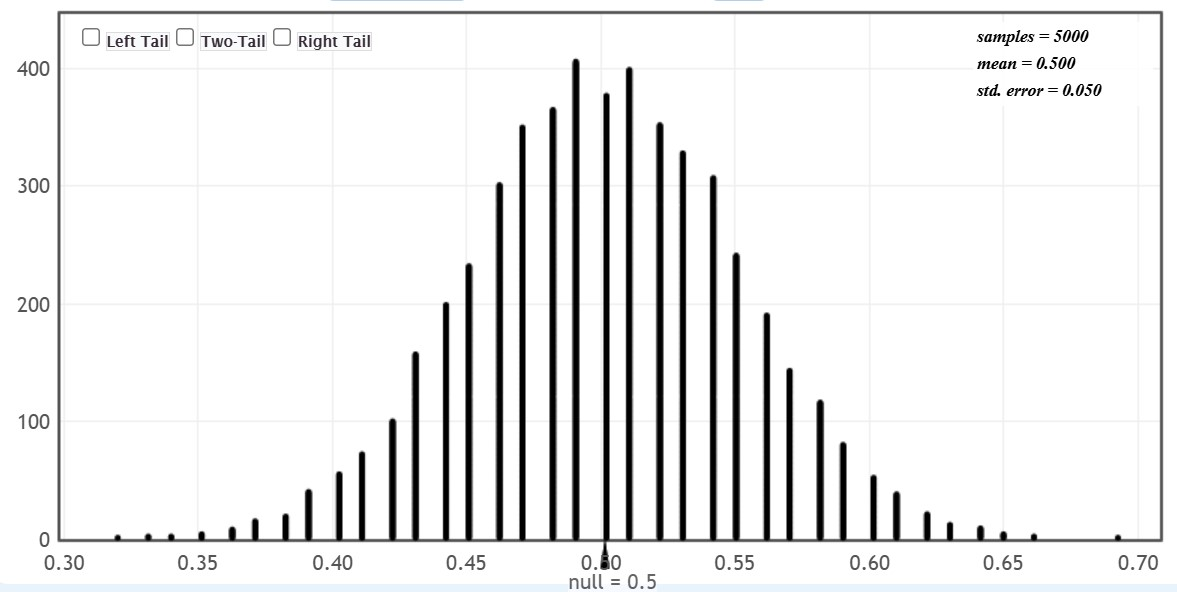
\includegraphics[scale=.55]{img/coin_null_distr2.jpg}
\end{center}
\begin{itemize}
    \item What do we see?
    \item Are large or small values of $\hat{p}$ more/less common?
\end{itemize}
\end{frame}

%%%%%%%%%%%%%%%%%%%%%%%%%%%%%%%%%%%%%%%%%%%%%%%%%%%%%%%%%%%%%%%%%
\begin{frame}{Null Distribution}
The \textbf{null distribution} will look very similar to the sampling distribution stuff we saw before
\begin{itemize}
    \item this time it is simulating the null hypothesis
    \item for means and proportions this looks like a Normal curve
\end{itemize} \vspace{8mm}

These distributions looks Normal when certain conditions are met. Very similar to what we had when we were using confidence intervals.
\end{frame}

%%%%%%%%%%%%%%%%%%%%%%%%%%%%%%%%%%%%%%%%%%%%%%%%%%%%%%%%%%%%%%%%%
\begin{frame}{Null Distribution -- Proportion}
Conditions:
\begin{itemize}
    \item Random Sample
    \begin{itemize}
        \item this doesn't affect our null distr. but makes sure answers are accurate
    \end{itemize}
    \item np$_0 >$ 10
    \item n(1 - p$_0) >$ 10
\end{itemize} \vspace{4mm}

With the conditions met, the null distribution for $\widehat{p}$ looks like this:
\begin{align*}
    \widehat{p} \sim N(p_0, \sqrt{\frac{p_0(1 - p_0)}{n}})
\end{align*}
\begin{itemize}
    \item use pnorm() to get p-values with these values for mean \& std. dev.
\end{itemize} \vspace{2mm}
\textbf{Note:} we have p$_0$'s in the distribution because we are simulating what the null hypothesis looks like
\end{frame}

%%%%%%%%%%%%%%%%%%%%%%%%%%%%%%%%%%%%%%%%%%%%%%%%%%%%%%%%%%%%%%%%%
\begin{frame}{Test Statistics}
\begin{align*}
    \widehat{p} \sim N(p_0, \sqrt{\frac{p_0(1 - p_0)}{n}})
\end{align*}

The test-statistic saves us from having to plot this Normal distribution every time. We will \textit{standardize} $\hat{p}$ to make the distribution simpler.

\begin{align*}
    \underbrace{\frac{\widehat{p}-p_0}{\sqrt{\frac{p_0(1 - p_0)}{n}}}}_{\text{Test Statistic}} \sim N(0,1)
\end{align*}
\begin{itemize}
    \item the whole term on the left is the Test-statistic
    \item we can compute this value and we know it follows N(0,1)
\end{itemize}
\end{frame}

%%%%%%%%%%%%%%%%%%%%%%%%%%%%%%%%%%%%%%%%%%%%%%%%%%%%%%%%%%%%%%%%%
\begin{frame}{Coin Flip Example}
For our scenario of 10 flips...
\begin{itemize}
    \item $\hat{p} = 8 / 10 = 0.8$
    \item $p_0$ = 0.5
    \item $\sqrt{\frac{p_0(1 - p_0)}{n}} = \sqrt{\frac{0.5(1 - 0.5)}{10}} = 0.158$
\end{itemize}
\begin{center}
    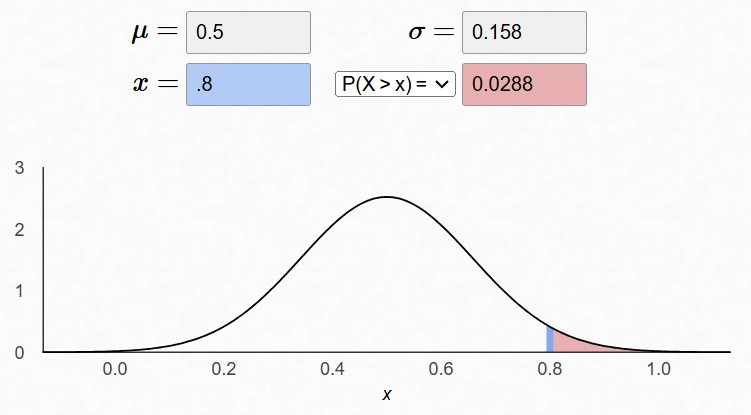
\includegraphics[scale=.65]{img/coin_null_distr3.jpg}
\end{center}
\begin{itemize}
    \item can use Null distr. and $\hat{p}$ to get p-value
\end{itemize}

\end{frame}

%%%%%%%%%%%%%%%%%%%%%%%%%%%%%%%%%%%%%%%%%%%%%%%%%%%%%%%%%%%%%%%%%
\begin{frame}{Coin Flip Example}
For our scenario of 10 flips...
\begin{itemize}
    \item $\hat{p} = 8 / 10 = 0.8$, $p_0$ = 0.5
    \item Z = $\frac{\widehat{p}-p_0}{\sqrt{\frac{p_0(1 - p_0)}{n}}} = \frac{0.8-0.5}{\sqrt{\frac{0.5(1 - 0.5)}{10}}} = 1.897$
\end{itemize}
\begin{center}
    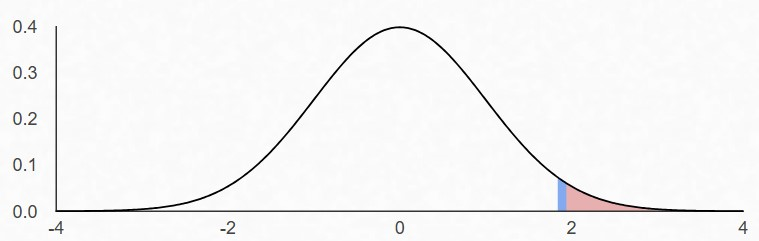
\includegraphics[scale=.75]{img/coin_null_distr4.jpg}
\end{center}
\begin{itemize}
    \item can use N(0,1) and Test-statistic Z to get p-value
\end{itemize}
\end{frame}

%%%%%%%%%%%%%%%%%%%%%%%%%%%%%%%%%%%%%%%%%%%%%%%%%%%%%%%%%%%%%%%%%
\begin{frame}{Test-statistics}
From here on out, we will place almost all of our emphasis on Test-statistics instead of elaborately detailing what the null distribution should look like.
\end{frame}

%%%%%%%%%%%%%%%%%%%%%%%%%%%%%%%%%%%%%%%%%%%%%%%%%%%%%%%%%%%%%%%%%
\begin{frame}{More on P-values}
Forms of the Alternate Hypothesis
\begin{itemize}
    \item H$_A$: parameter $>$ 'hypothesized value' (right-tailed test) \textbf{\underline{OR}}
    \item H$_A$: parameter $<$ 'hypothesized value' (left-tailed test) \textbf{\underline{OR}}
    \item H$_A$: parameter $\neq$ 'hypothesized value' (two-tailed test)
\end{itemize} \vspace{6mm}

Up until now we have only seen how to calculate p-values Alternate Hypotheses that use the $>$ symbol.
\begin{itemize}
    \item coin flip biased in favor of heads ($H_A:$ p $> 0.5$)
    \item Monday breakups ($H_A$: p $> \frac{1}{7}$)
\end{itemize}
    
\end{frame}

%%%%%%%%%%%%%%%%%%%%%%%%%%%%%%%%%%%%%%%%%%%%%%%%%%%%%%%%%%%%%%%%%
\begin{frame}{More on P-values}
H$_A$: parameter $>$ 'hypothesized value' (right-tailed test)
\begin{itemize}
    \item to find a p-value, you find where the Test-statistic is on a N(0,1) distribution, then find the area to the right of it under the curve
\end{itemize} \vspace{2mm}

Suppose test-stat Z = 1.9
\begin{center}
    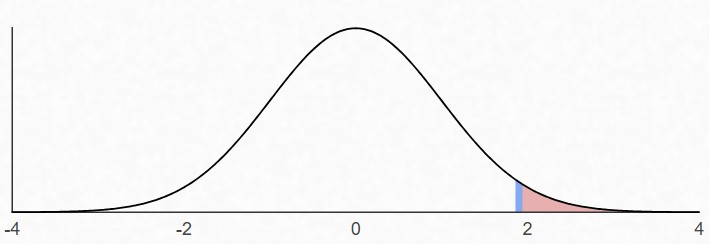
\includegraphics[scale=.7]{img/standardnormal_pvalue1.jpg}
    
    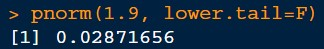
\includegraphics[scale=1]{img/Rpval1.jpg}
\end{center}
\end{frame}

%%%%%%%%%%%%%%%%%%%%%%%%%%%%%%%%%%%%%%%%%%%%%%%%%%%%%%%%%%%%%%%%%
\begin{frame}{More on P-values}
H$_A$: parameter $<$ 'hypothesized value' (left-tailed test)
\begin{itemize}
    \item to find a p-value, you find where the Test-statistic is on a N(0,1) distribution, then find the area to the left of it under the curve
\end{itemize} \vspace{2mm}

Suppose test-stat Z = -.5
\begin{center}
    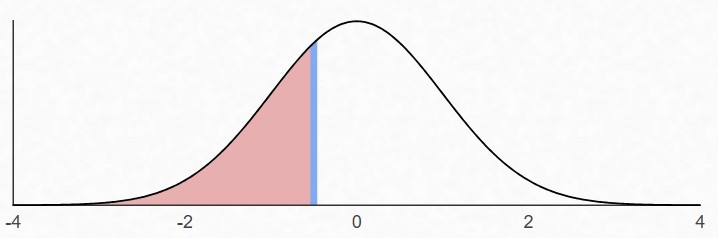
\includegraphics[scale=.7]{img/standardnormal_pvalue2.jpg}

    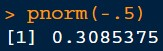
\includegraphics[scale=1]{img/Rpval2.jpg}
\end{center}
\end{frame}

%%%%%%%%%%%%%%%%%%%%%%%%%%%%%%%%%%%%%%%%%%%%%%%%%%%%%%%%%%%%%%%%%
\begin{frame}{More on P-values}
H$_A$: parameter $\neq$ 'hypothesized value' (two-tailed test)
\begin{itemize}
    \item to find a p-value, you find where the Test-statistic is on a N(0,1) distribution
    \item area to the right (Test-stat $>$ 0) or area to the left (Test-stat $<$ 0)
    \item multiply this area by 2
\end{itemize} \vspace{2mm}

Suppose test-stat Z = 1
\begin{center}
    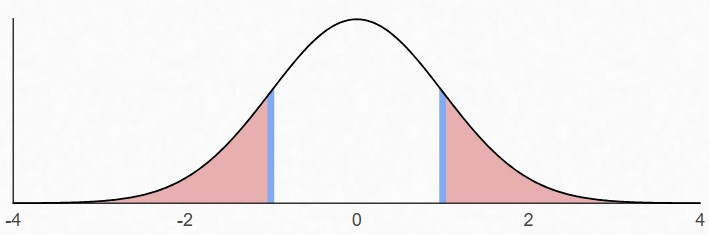
\includegraphics[scale=.7]{img/standardnormal_pvalue3.jpg}
    
    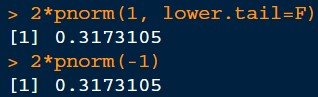
\includegraphics[scale=1]{img/Rpval3.jpg}
\end{center}
\end{frame}

\end{document}